\chapter{Návrh riešenia problému}
\section{Existujúce problémy}
Pred zahájením tvorby aplikácie je nutné oboznámiť sa s problémami, ktoré je nutné aby aplikácia riešila. Na prvý pohľad  sa môže zdať, že  počítanie ľudí je jednoduchý proces. Predpokladajme, že virtuálna brána je umiestnená pri vstupe do miestnosti. Proces prechodu osoby znamená zvýšenie počítadla prechodov osôb a na základe smeru danej osoby dekrementovať alebo inkrementovať počet osob nachádzajúcich sa v miestnosti. Systém musí byť navrhnutý tak, aby bol schopný detekovať a sledovať aj viacero ľudí ktorý v jedenom okamihu prechádzajú cez virtuálnu bránu rovnakým alebo odlišným smerom.  Jeden z najväčších problémov je však dynamickosť prostredia, kde by aplikácia mala byť nasadená. Rýchle svetelné zmeny okolia,  nepredvídateľné pohyby ľudí na scéne (môže zastať, dotýkať sa, ťahať / tlačiť iný objekt)  toto všetko je nutné riešiť, tak aby aplikácia dosiahla čo najväčšej presnosti. 

\section{Konceptuálny návrh systému}
Z problémov opísaných v sekcii 3.1 je jasné, že jednoduché systémy typu Infračervená závora, nebudú mať dostatočne veľkú presnosť vzhľadom na prechody viacerých osôb v jednom časovom okamihu. Je nutné oprieť sa o metódy, ktoré vedia zaznamenať viac informácii o objekte, ktorý prechádza vymedzeným priestorom (tvar, rýchlosť, veľkosť, smer, atd …). 

Jedným z najkomplexnejších prostriedkov, ako dostať dáta do počítača na spracovanie je kamera, ktorá nám poslúži ako senzor.  Umiestnime ju na vrchnú priečku prechodu tak, aby snímala osoby z vrchu. Táto pozícia je najlepšia, lebo eliminuje možnosti zatienenia sledovaného objektu iným objektom na scéne.  

\begin{figure}[H]
  \centering
  \begin{minipage}[b]{0.2\textwidth}
    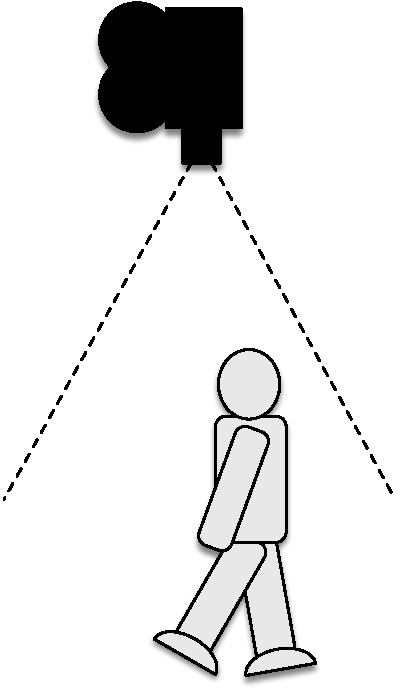
\includegraphics[width=\textwidth]{obrazky/konceptSnimania}
    \caption{Poloha kamery.}
  \end{minipage}
  \hfill
  \begin{minipage}[b]{0.5\textwidth}
    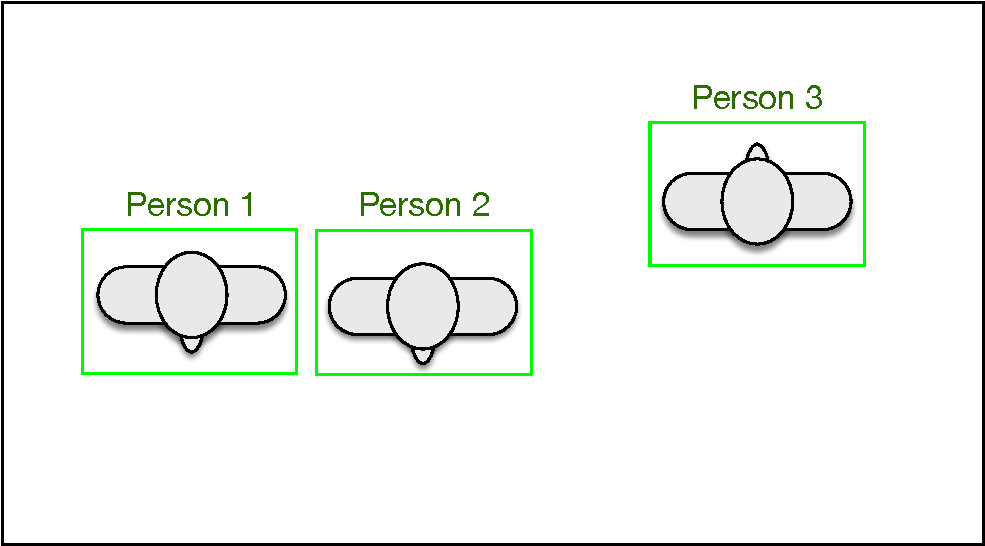
\includegraphics[width=\textwidth]{obrazky/pohladZhora}
    \caption{Obraz snímanej scény}
  \end{minipage}
\end{figure}

\section{Výber snezora (kamery)}
Výber vhodného snímača priestoru virtuálnej brány je veľmi dôležitý. Ak senzor bude snímať dáta, ktoré sú enormne zaťažené šumom, realizácia funkčného algoritmu bude veľmi náročná, v niektorý prípadoch až nemožná. Táto práca sa zameriava na dva typy vhodných kamier \textbf{3D kamery} a\textbf{ 2D  RGB kamery}.

\subsection{3D kamery}
Keďže  koncept snímania priestoru sa opiera o snímanie z výšky, veľmi silným kandidátom sú aktívne 3D kamery. Veľká výhoda je meranie na základe tvorby hĺbkového obrazu(kapitola XXX). Vďaka tomu, má meranie vysokú presnosť, nepotrebuje osvetlenie priestoru ani kontrastné prostredie.  Ďalšou veľkou výhodov je informácia o výške osoby, ktorá prechádza. Táto informácie je použiteľná v mnohých aspektoch ďalšieho spracovania. Na druhej strane technológia aktívneho 3D hĺbkomera je náchylná na priame slnečné lúče. Tie dokážu merania veľmi znehodnotiť. Vo svojej práci som otestoval tri rôzne aktívne hĺbkomery: 

\begin{itemize}
\item Kinect 360
\item Orbbec Astra S
\item Intel RealSence SR300

\end{itemize}

\subsubsection{Testovanie}
Testovanie spočívalo v umiestnení všetkých troch kamier na vhodné miesto, kde sa nahrával záznam po dobu 10 minút. Vďaka tomu je zaručené, že všetky tri kamery boli vystavené rovnakému prostrediu a boli nahrávané za rovnakých svetelných podmienok.  Počas nahrávania bol udržiavaný konštantný pohyb osôb cez bránu. Pre ohodnotenie kvality jednotlivých záznamov bola použitá \textbf{metrika hodnotenia} založená na priemernom počte nenameraných pixelov na jednom snímku. Nenameraný pixel znamená, že sa nachádza nekonečne ďaleko alebo ide o chybu merania spôsobená tvarom objektu (ostrá hrana), slnečným žiarením, materialom oklitého prostredia alebo iné. \textit{Metóda pre výpočet hodnotiacej metriky konverguje k objektívnemu výsledku len vtedy, ak každý objekt scény sa nachádza v zornom poli kamery, ktoré udáva jej výrobca.}  

\subsubsection{Kinect 360}
Kinect sníma frekvenciou 30 Hz. Hĺbka je snímaná s presnosťou na 11 bitov, čiže hĺbka jedného pixela môže nadobudnúť hodnoty od 0 do 2047.  Pracovný rozsah senzora je  1,2 - 3,5 metra.  Využíva technológiu vyvinutú firmou PrimaSence. V ľavej časti senzora sa nachádza IR projektor s vlnovou dĺžkou svetla 830nm. Generátor kóduje informáciu do svetelných vzorov, ktoré sa odrazom od predmetov pred senzorom deformujú. Odraz IR svetla je zachytený senzorom v pravej časti senzora a z veľkosti deformácii je vypočítaná hĺbková mapa. Používa USB 2.0 rozhranie. 

Kedže od spoločnosti Microsoft neexistuje oficialna podpora operačných systémov Unixového typu, na čítanie obrazu z kameri som použil knižnicu vyvíjanú komunitou \textit{libfreenect}. Tú som testoval na RaspberryPI v3 s opereačným systémom Rasbian a MacOS Sierra. Na oboch operačných systémoch fungovala dobre pekne pri 20 až 25 FPS. 

Veľkým problémom pri používaní tohoto hĺbkomeru je jeho veľkosť, váha, nutnosť externého napájania. Ďalší problém sa týka dostupnosti senzora. Senzor je zastaralí a už sa nevyrába. Cena sa momentálne stále drží na úrovni 150 eur. 

\subsubsection{Orbbec Astra S}
Ide o kameru, ktorá má veľmi podobný princíp funkčnosti ako kinect, čiže technológia je založená na vysielaní štrukturovaného svetla. Pracovný rozsah senzora je 0.4 – 2 metra. Kamera je pomerne malá a nepotrebuje externé napájanie. Používa USB 2.0 rozhranie. 

Knižnice od spoločnosť Orbbec má veľmi dobrú podporu všetkých operačných systémov. Cena 150 eur. 


\subsubsection{Intel RealSence SR300}
Je kamera, ktorá sa pomerne dosť líši od predchádzajúcich dvoch. Hlavným rozdielom je, že používa USB 3.0 čo znamená, že posiela väčšie množstvo dát a nieje možné ho pripojiť na RaspberyPi. Technológia snímania je založená na štrukturovanom svetle, podobne ako v predchádzajúcich dvoch prípadoch. Pracovný rozsah kamery je 25 až 70 cm. Cena kamery je tiež okolo 150 eur. 

\subsubsection{Porovnanie}
Prvým parametrom porovnávania je \textbf{zorné pole kamier}. Každá hĺbková kamera, podobne ako klasické RGB kamery, majú zorný uhol daný použitou optikou kamery, hĺbkomery však majú navyše atribúty maximálnej a minimálnej vzdialenosti, na ktoré sú schopné vykonať meranie. Je to z dôvodu primárneho použiria kamery, pre ktoré ho výrobca vyrába. Napriklad \textit{Kinect 360} je určený pre hernú konzolu a detekciu celého tela, preto ma zorné pole veľmi veľké, aby mal hráč aj istú dávku voľnosti v pohybe. Presný opak kamery Kinect predstavuje \textit{Intel RealSence} ktorá je určená na aplikácie ovládania PC rôznymi gestami. Z dôvodu takéhoto obmedzenia nieje možné postaviť aplikáciu sledovania prechodov ľudí na jednom type kamery. (OBR 3.3) 

Fyzické okolie virtuálnej brány nemusí dovoľovať umiestniť hĺbkomer do požadovanej snímacej výšky. Preto najlepším spôsobom je vyberať senzor špeciálne pre každé miesto nasadenia. Vďaka tomu je možné realizovať meranie od 2m do 4,5m.

\begin{figure}[H]
\begin{center}
	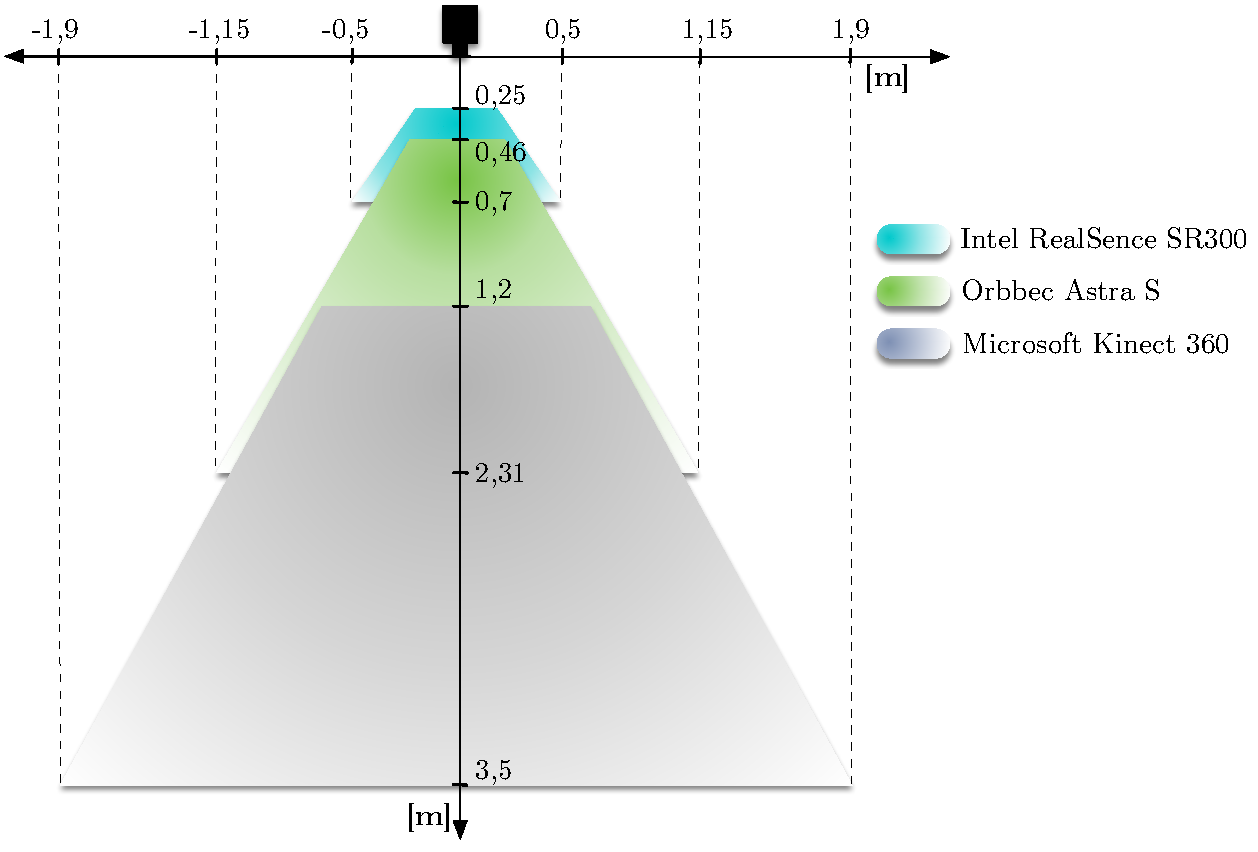
\includegraphics[scale=0.7]{obrazky/camerasViews}
	\caption{Vizualizácia vertikálneho zorného pola hĺbkomerov}
	\end{center}
\end{figure}
























